\documentclass{templates/fhnwreport}

\graphicspath{{./resources/}{../resources/}}

\begin{document}

% **************************************************************************** %
% Title
% **************************************************************************** %
\project{Bildverarbeitung}
\title{
  Laborbericht\\[.5em]
  Bildverarbeitungslabor  
}
\author{
  Alex Murray, Simon Sturm, Florian Wernli\\
  Elektro- und Informationstechnik\\
  Fachhochschule Nordwestschweiz\\
}

\supervisor{Betreuer: Stefan Umbricht, Jürg P. Keller}

\maketitle

\clearpage
\pagestyle{empty}
{
  \tableofcontents
}

\clearpage
\pagestyle{fancy}
\section{Schärfe \& Lichtmenge}
\subsection{Theoretische Grundlagen}
Die Schärfentiefe (engl. depth of field (DOF)) beschreibt die Distanz,
beziehungsweise einen Entfernungsbereich,
in welcher ein Objekt scharf abgebildet wird.

\begin{figure}[h!]
  \centering
  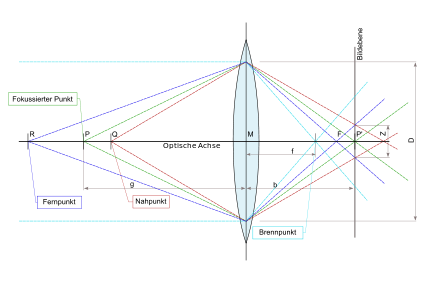
\includegraphics[width=.6\textwidth]{Posten_1_theo}
  \caption{Strahlengänge zur Bestimmung der Schärfentiefe mit Fernpunkt im Endlichen \cite{ref:wiki:schaerfentiefe}}
  \label{fig:p1theo}
\end{figure}

Zur Berechnung der Schärfentiefe werden die Brennweite $f$, die Blendenzahl $k$,
die Gegenstandsweite $g_s$ und die grösse des Zerstreuungskreis $Z$ benötigt.
Wie in Abbildung \ref{fig:p1theo} ersichtlich, gibt der Zerstreuungskreis $Z$ an,
wie gross eine Punktquelle auf der Bildebene abgebildet wird.
Da die Bildebene mit der Auflösung des Bildsensors abgetastet wird,
sind Kreise kleiner als die Pixelgrösse kaum wahrnehmbar,
das heisst die Aufnahme wird noch immer scharf.

Für die Bestimmung der Schärfentiefe, respektive des Nah- und Fernpunktes,
wird die hyperfokale Entfernung benötigt.
Diese beschreibt, auf welche endliche Entfernung fokusiert werden muss,
so dass der Fernpunkt im Unendlichen liegt.

\begin{equation}
  g_h=\frac{f^2}{kZ}+f
\end{equation}

Der Nahpunkt lässt sich wie folgt berechnen: 
\begin{equation}
  g_n=\frac{g_s}{1+\frac{g_s-f}{g_h-f}}
\end{equation}

Die Berechnung der Fernpunkts benötigt nur eine Anpassung eines Vorzeichens:
\begin{equation}
  g_f=\frac{g_s}{1-\frac{g_s-f}{g_h-f}}
\end{equation}

\newpage
\subsection{Versuchsaufbau}
Benötigtes Material:
\begin{itemize}
\item Kamera Basler A1300-30gc
\item Objektiv Computar 25mm f1.4:16
\item Objektiv Computar 16mm f2:16
\end{itemize}

Der Studentenausweis wird wie in Abbildung \ref{fig:p1auf} vor der Kamera aufgestellt.
Mit beiden Objektiven wird die Schärfentiefe mit unterschiedlichen Blendenstufen untersucht.

\begin{figure}[h!]
  \centering
  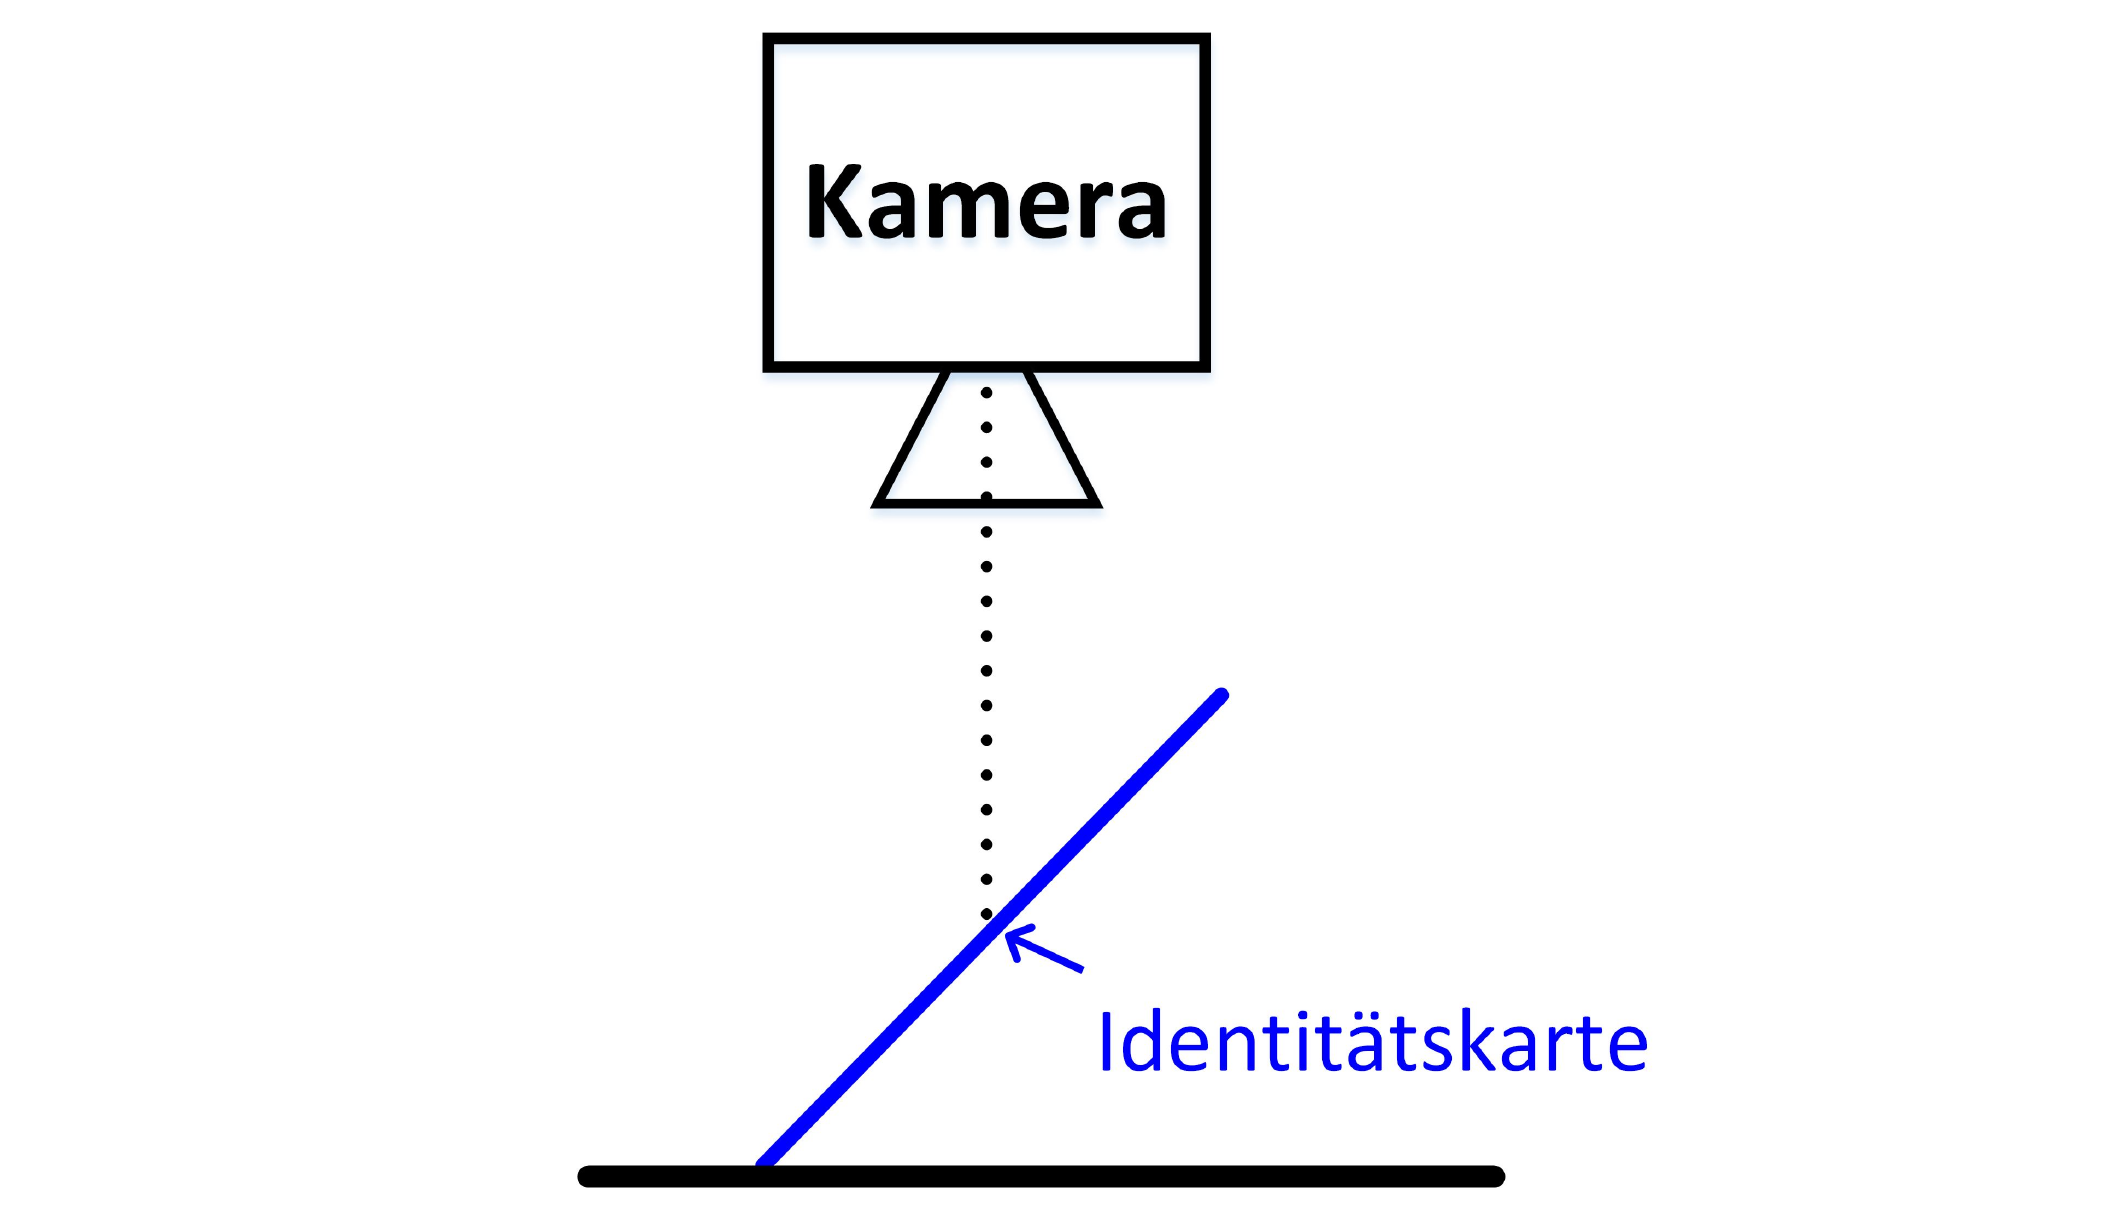
\includegraphics[width=.6\textwidth]{Posten_1_aufbau}
  \caption{Versuchsaufbau \cite{ref:bver:stefan}}
  \label{fig:p1auf}
\end{figure}

\subsection{Ergebnisse}
\subsubsection{Testbild mit Brennweite 25mm und f1.4}
\begin{wrapfigure}[5]{L}{.6\textwidth}
  \centering
  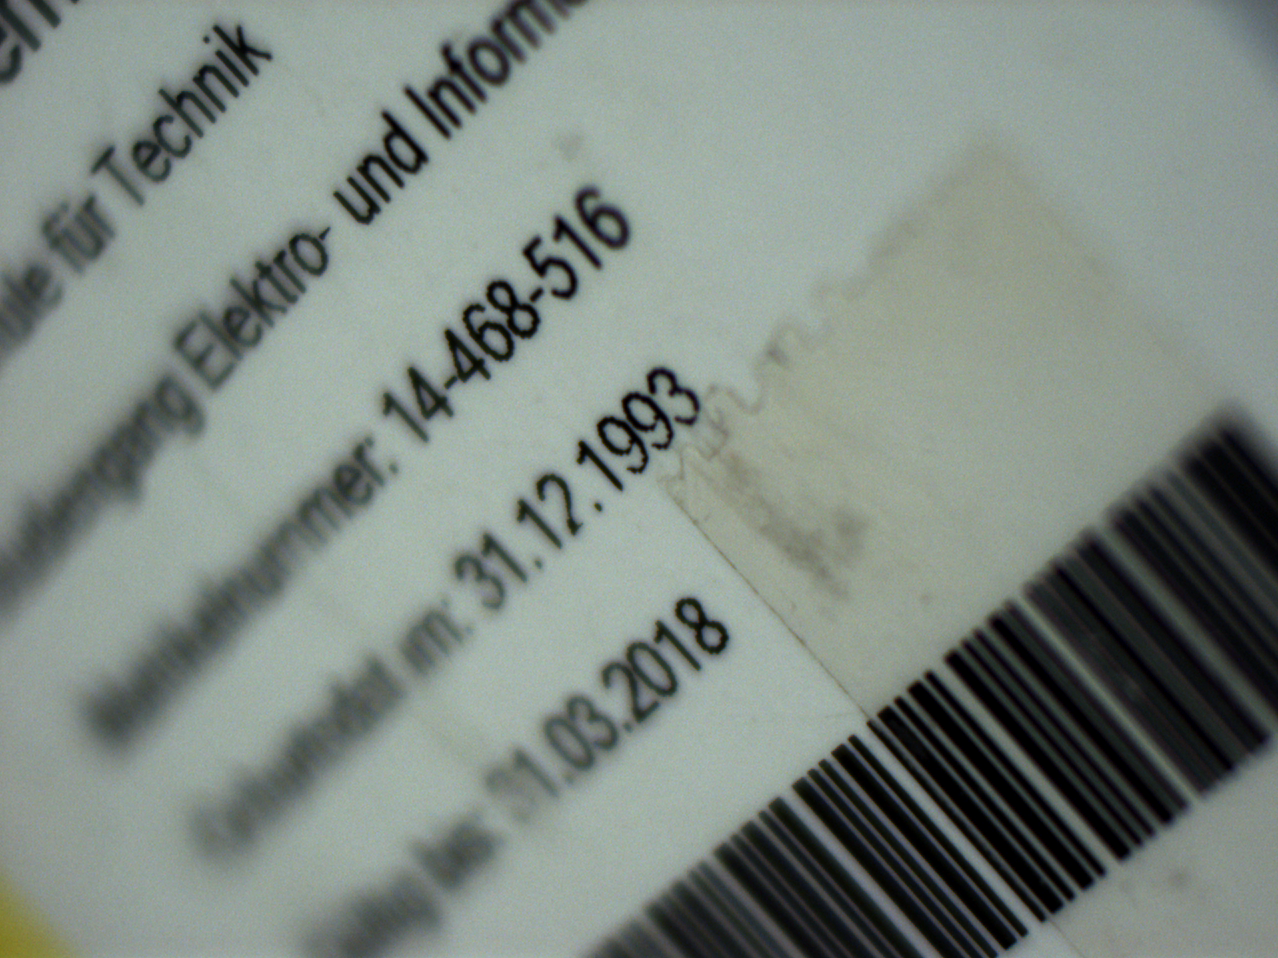
\includegraphics[width=.6\textwidth]{Posten_1_img_1}
  \caption{Studentenausweis mit Brennweite 25mm f1.4}
  \label{fig:b25f1.4}
\end{wrapfigure}

~\\[2em]
Einstellungen:\\
\begin{tabular}{l l}
  Brennweite $f$:        &  $25$mm\\
  Blendenzahl $k$:       & 1.4 \\
  Distanzscharf $g_s$    & 140mm \\
  Zerstreuungskreis $Z$: & $0.00375$mm\\
\end{tabular}

~\\[10em]

\[
  g_h=\frac{25^2}{0.00375*1.4}+25=119072.61904\;\text{mm}
\]
\[
  g_n=\frac{140}{1+\frac{140-25}{g_h-25}}=139.86\;\text{mm}
\]
\[
  g_f=\frac{140}{1-\frac{140-25}{g_h-25}}=140.14\;\text{mm}
\]

\subsubsection{Testbild mit Brennweite 16mm und f2}
  \begin{wrapfigure}[5]{L}{.6\textwidth}
    \centering
    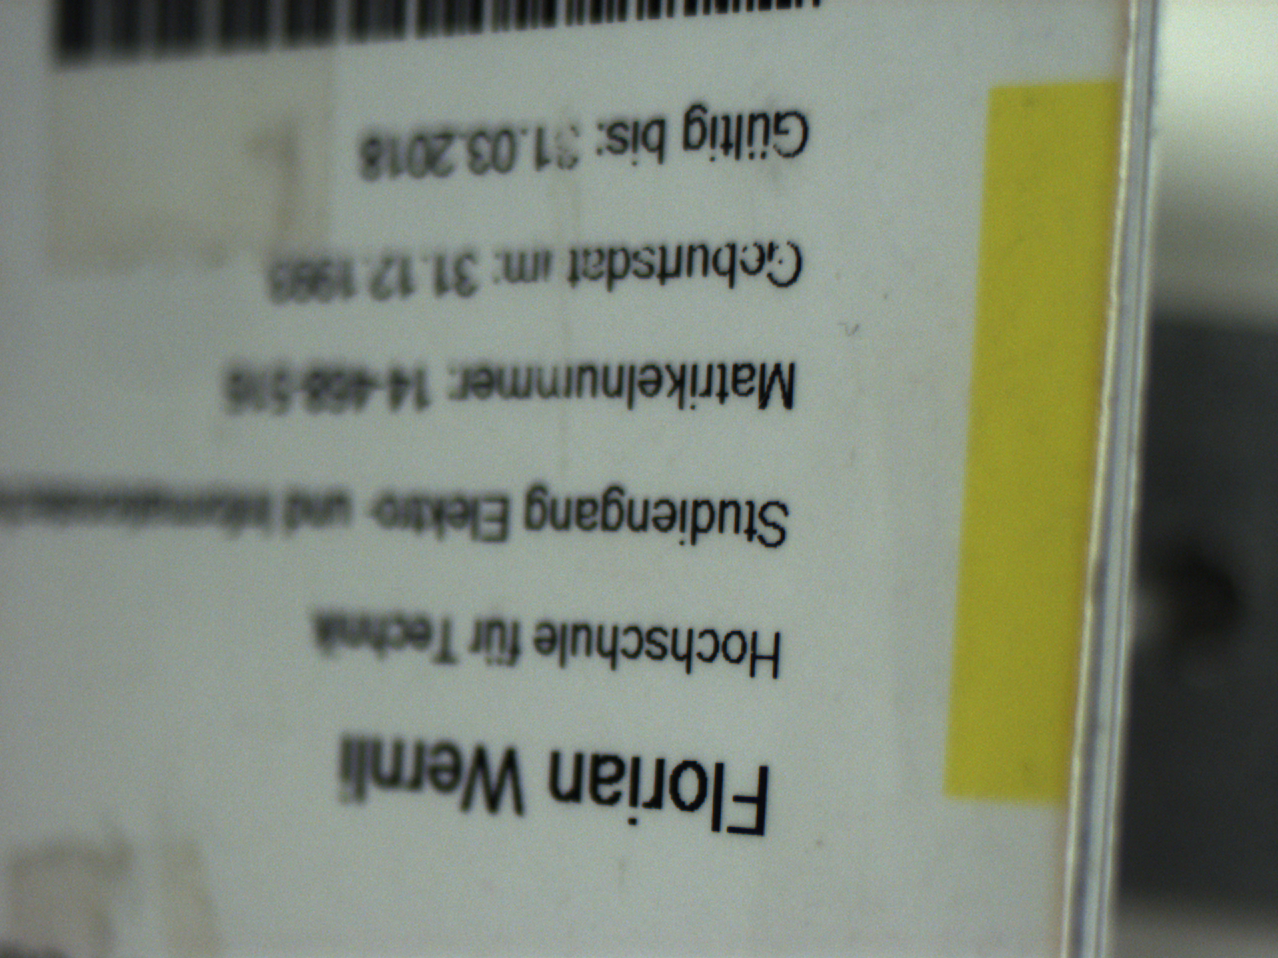
\includegraphics[width=.59\textwidth]{Posten_1_16mm_1}
    \caption{Studentenausweis mit Brennweite 16mm f2}
    \label{fig:b25f2}
  \end{wrapfigure}

  ~\\[2em]
  Einstellungen:\\
  \begin{tabular}{l l}
    Brennweite $f$:        & $16$mm\\
    Blendenzahl $k$:       & 2 \\
    Distanzscharf $g_s$    & 140mm \\
    Zerstreuungskreis $Z$: & $0.00375$mm\\
  \end{tabular}

  ~\\[10em]

\[
  g_h=\frac{16^2}{0.00375*2}+16=34149.3333\;\text{mm}
\]
\[
  g_n=\frac{140}{1+\frac{140-16}{g_h-16}}=139.49\;\text{mm}
\]
\[
  g_f=\frac{140}{1-\frac{140-16}{g_h-16}}=140.51\;\text{mm}
\]

\subsection{Erkenntnisse}

Die Schärfentiefe ist bei weit entfernten Objekten grösser, da die eingestellte Schärfe sich der hyperfokalen Entfernung nähert, beziehungsweise der Einfallswinkel der Strahlen weniger stark mit der Distanz variiert.

Der Versuch zeigt sehr gut, dass eine Verbesserung der Schärfentiefe durch die Verkleinerung der Blendenöffnung erfolgen kann.
Die künstliche Vignettierung verkleinert den Unschärfekreis.
Da aber weniger licht auf den Sensor fällt, muss das Signal mehr verstärkt werden,
wodurch das Rauschen erhöht wird.

Nicht direkt aus dem Versuch aber aus der Formel ist ersichtlich, dass eine kleiner die Brennweite der Optik und damit ein kleiner der Sensor positiv zur Schärfentiefe beitragen, ebenso wie eine grössere Pixelgrösse.

\clearpage
\section{Brennweite}
\subsection{Theoretische Grundlagen}

Die Funktionsweise  der meisten Digitalkameras kann anhand eines Linsensystems
erkl\"art werden, der ein Gegenstand auf ein CCD (engl. \textit{Charge Coupled
Device})  auch  \textit{Bildsensor}  gennant,  projeziert   (siehe   Abbildung
\ref{fig:linseccd}).

\begin{figure}[h!]
    \centering
    \begin{subfigure}[b]{.45\linewidth}
        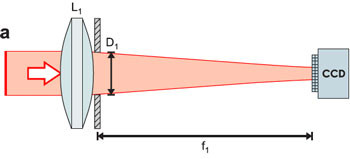
\includegraphics[width=\textwidth]{imLinseCCD}
        \caption{Linse, die ein Gegenstand auf den Kamerasensor abbildet \cite{ref:perfektfokusiert}}
        \label{fig:linseccd}
    \end{subfigure}
    \begin{subfigure}[b]{.45\linewidth}
        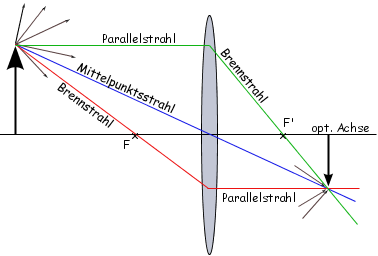
\includegraphics[width=\textwidth]{imLinsengleichung}
        \caption{Eine Visualisierung der Linsengleichung \cite{ref:Linsengleichung}}
        \label{fig:linsengleichung}
    \end{subfigure}
\end{figure}

Sind die physikalischen Dimensionen  dieses Sensors bekannt, so kann mit Hilfe
der Linsengleichung  (siehe  Abbildung \ref{fig:linsengleichung} und Gleichung
\ref{eq:linsengleichung}) das Linsensystem berechnet werden und somit von  der
Bildgr\"osse    auf    der    realen    Gegenstandsgr\"osse   eines   Objektes
zur\"uckgeschlossen werden. Die Linsengleichung lautet:

\begin{equation}
    \frac{1}{f} = \frac{1}{g} + \frac{1}{b}
    \label{eq:linsengleichung}
\end{equation}

Weiter kann der Vergr\"osserungsfaktor $\beta$ berechnet werden:

\begin{equation}
    \beta = \frac{B}{G} = \frac{b}{g}
\end{equation}


\subsection{Versuchsaufbau}

Nenndaten der Kamera:
    
\begin{itemize}
    \item Aufl\"osung Sensor : 1024x768 Pixel
    \item Gegenstandsweite : \SI{13}{\centi\meter}
    \item Cell Size : \SI{4.65 x 4.65}{\micro\meter}
    \item Brennweite : \SI {6}{\milli\meter}
\end{itemize}

Der  Studentenausweis  wird  direkt  von  Oben  fotografiert  und die  Distanz
zwischen   der   Linse    und    des    Studentenausweises    wird    gemessen
(\SI{13}{\centi\meter}).


\subsection{Ergebnisse}

\begin{figure}[h!]
    \centering
    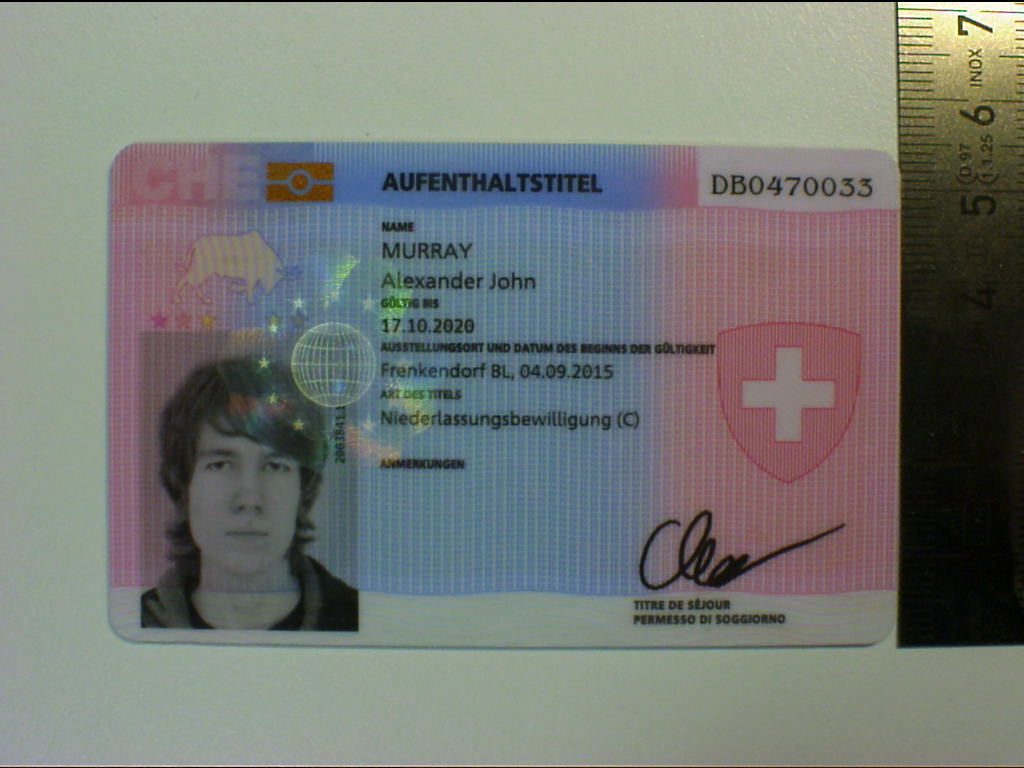
\includegraphics[width=.6\linewidth]{Posten_2_fuckface.png}
    \caption{Aufgenommenes Bild des Studentenausweises}
\end{figure}

Die Dimensionen  in  Pixel des Aufgenommenn Studentenausweises wurde mit einem
Bildverarbeitungsprogramm ermittelt. Sie ergibt sich als 787 x  511  Pixel. Da
die  Sensoraufl\"osung bekannt ist (1024 x 786 Pixel) sowie auch die Cell Size
(\SI{4.65  x  4.65}{\micro\meter})  kann  die Abbildungsgr\"osse des Ausweises
berechnet werden.

\begin{align*}
    B_x = 787\cdot\SI{4.65}{\micro\meter} &= \SI{3659.55}{\micro\meter} \\
    B_y = 511\cdot\SI{4.65}{\micro\meter} &= \SI{2376.15}{\micro\meter}
\end{align*}

Der  Abstand  zum  Brennpunkt  $f$  ist  in   den  Nenndaten  der  Kamera  als
\SI{6}{\milli\meter} angegeben. Der Abstand zum Gegenstand $g$ wurde gemessen.
So    kann    die    Abbildungsabstand    $b$    mit    der    Linsengleichung
(\ref{eq:linsengleichung}) berechnet werden.

\begin{equation*}
    b = \frac{1}{\frac{1}{f}-\frac{1}{g}} = \SI{6.29}{\milli\meter}
\end{equation*}

Mit $g$ und $b$ kann der Vergr\"osserungsfaktor $\beta$ berechnet werden:

\begin{equation*}
    \beta = \frac{b}{g} = 0.04838
\end{equation*}

Und folglich kann somit die Gegenstandsgr\"osse berechnet werden:

\begin{align*}
    G_x = \frac{B_x}{\beta} &= \SI{75.63}{\milli\meter} \\
    G_y = \frac{B_y}{\beta} &= \SI{49.11}{\milli\meter}
\end{align*}


\subsection{Erkenntnisse}

Die  berechnete Gegenstandsgr\"osse (\SI{49.11}{\milli\meter}) ist  ein  wenig
kleiner   als   die   gemessene  Gegenstandsgr\"osse  (\SI{54}{\milli\meter}).

Die  Ursache hierf\"ur kann  einerseits  auf  Ungenauigkeiten  der  gemessenen
Distanz $g$  zwischen  Gegenstand  und Linse zur\"uckgef\"uhrt werden (weil es
nicht ganz klar war wo die Linse im Objektiv anf\"angt), anderseits  kann  der
Fehler auch davon stammen, dass das Objektiv nicht nur aus einer Linse besteht
sondern aus einem Linsensystem.



\clearpage
\section{Beleuchtung \& Filter}
\subsection{Ringlicht}

Wird  ein  Objekt  von allen Seiten beleuchtet aber nicht von Oben, so  werden
Gravierungen sehr gut hervorgehoben (siehe Abbildung \ref{fig:muenzen}).

\begin{figure}[h!]
    \centering
    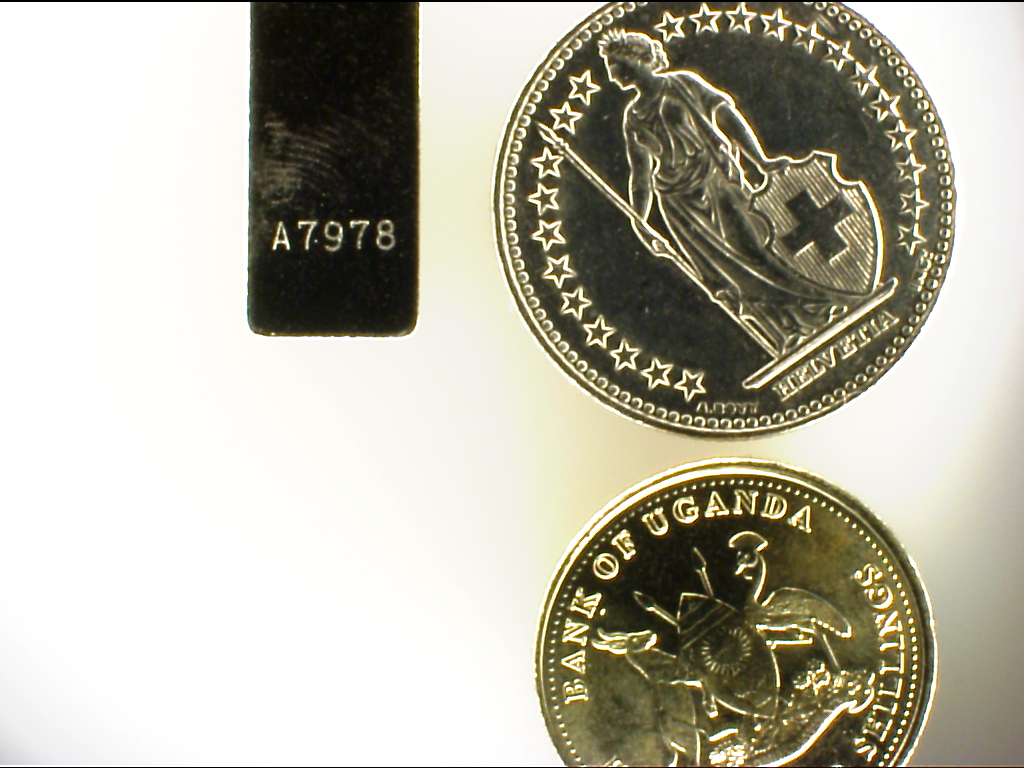
\includegraphics[width=.6\linewidth]{Posten_3_1_a_meme_1.png}
    \caption{Gravierungen sind sehr gut ersichtlich. Von Auge sieht man die Zahl ``A7978'' kaum.}
    \label{fig:muenzen}
\end{figure}


\subsection{Durchlichtbeleuchtung}

Mit Durchleuchtung  von Objekten lassen sich Materialien, die von Aussen nicht
sichtbar sind, hervorheben, weil  sie  das  durchleuchtende  Licht  blockieren
(siehe Abbildungen \ref{fig:note1} und \ref{fig:note2}).

\begin{figure}[h!]
    \centering
    \begin{subfigure}[b]{.45\linewidth}
        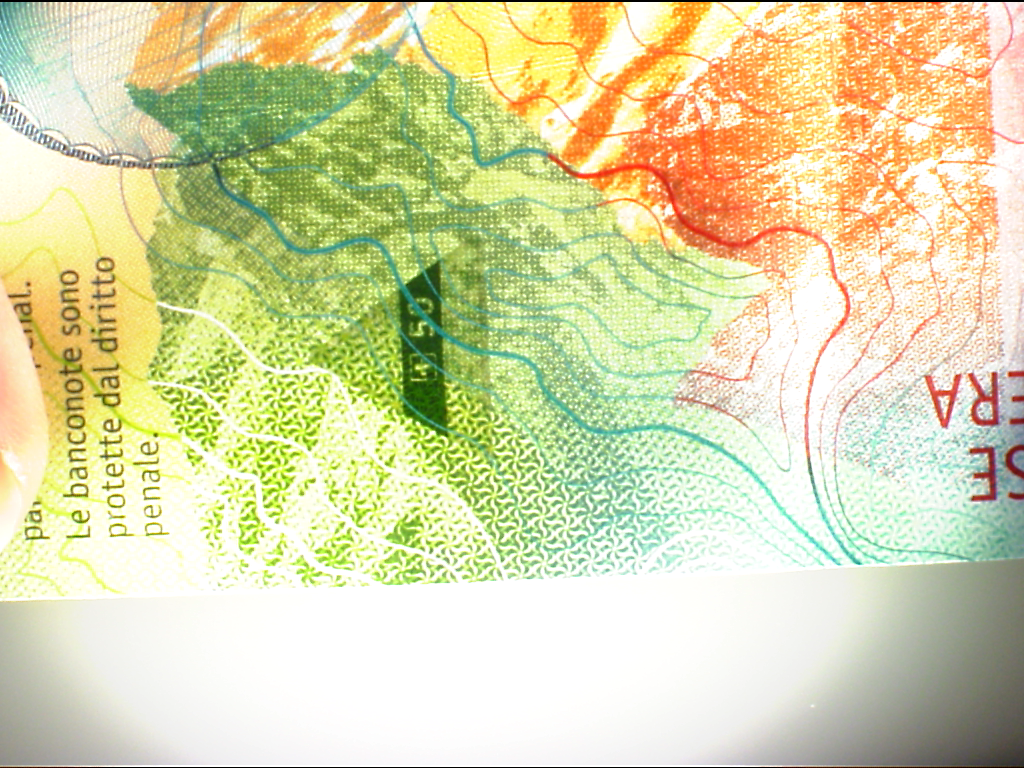
\includegraphics[width=\linewidth]{Posten_3_1_illuminati_invis}
        \caption{Das Band ist ohne Durchleuchtung nicht sichtbar.}
        \label{fig:note1}
    \end{subfigure}
    \begin{subfigure}[b]{.45\linewidth}
        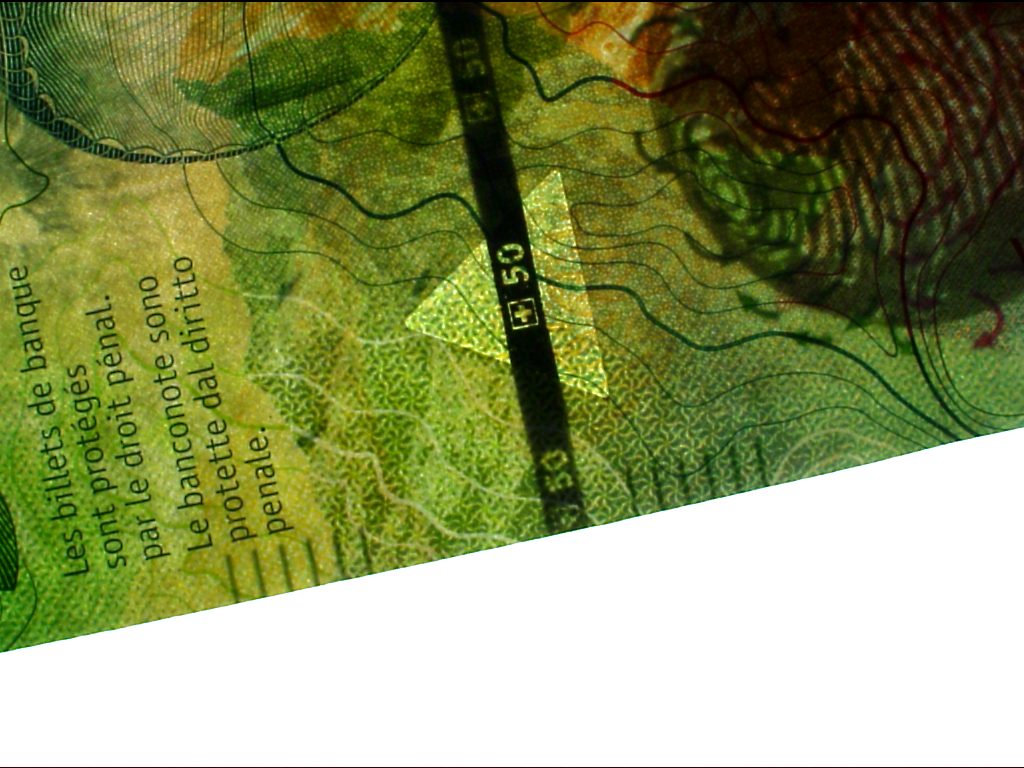
\includegraphics[width=\linewidth]{Posten_3_1_illuminati_visible}
        \caption{Mit Durchleuchtung wird das Band nun sichtbar.}
        \label{fig:note2}
    \end{subfigure}
\end{figure}


\newpage
\subsection{Polfilter}

Die  Lichtquelle   erzeugt   polarisiertes  Licht,  welches  von  der  M\"unze
reflektiert wird. Unter  Verwendung  eines  Polfilters kann das reflektierende
polarisierte Licht herausgefiltert werden.

\begin{figure}[h!]
    \centering
    \begin{subfigure}[b]{.45\linewidth}
        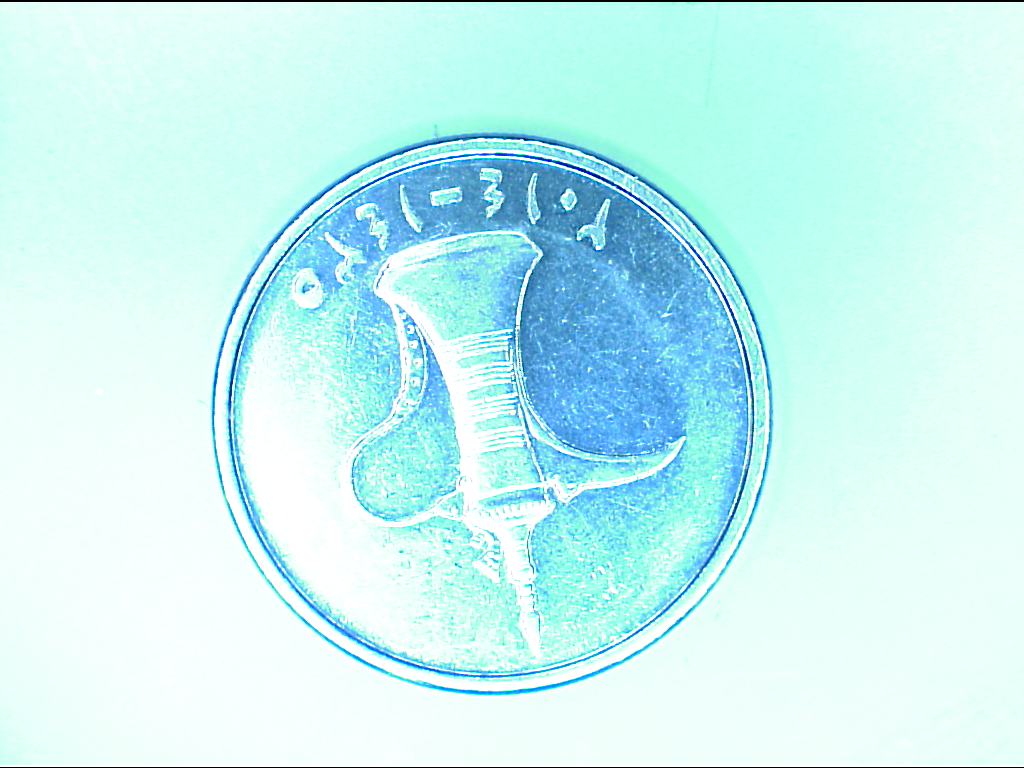
\includegraphics[width=\linewidth]{Posten_3_2_d_Reflektion_Stellung1}
        \caption{Ohne Polfilter}
    \end{subfigure}
    \begin{subfigure}[b]{.45\linewidth}
        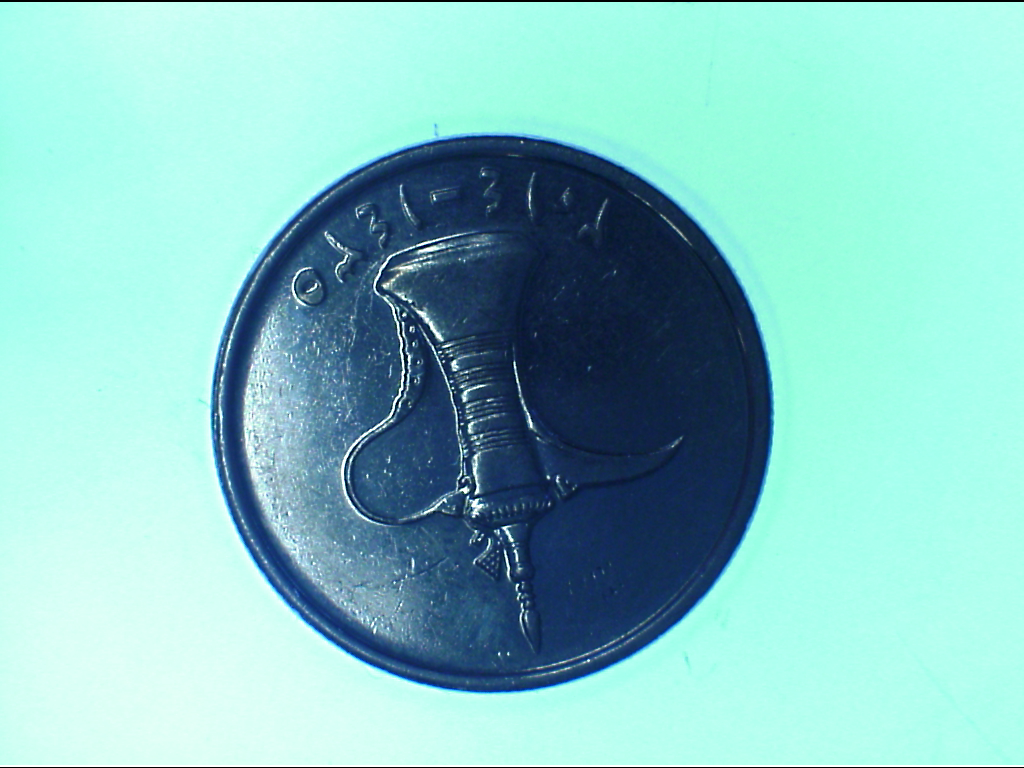
\includegraphics[width=\linewidth]{Posten_3_2_d_Reflektion_Stellung2}
        \caption{Mit Polfilter}
    \end{subfigure}
\end{figure}


\subsection{Dombeleuchtung}

Die  Dombeleuchtung  hebt  wie beim Ringlicht die Gravur der  M\"unze  hervor.
Dabei ist zu beachten dass kein Streulicht in  die  Dom  eindringt, was in den
Abbildungen \ref{fig:dom1} und \ref{fig:dom2} zu sehen ist.

\begin{figure}[h!]
    \centering
    \begin{subfigure}[t]{.45\linewidth}
        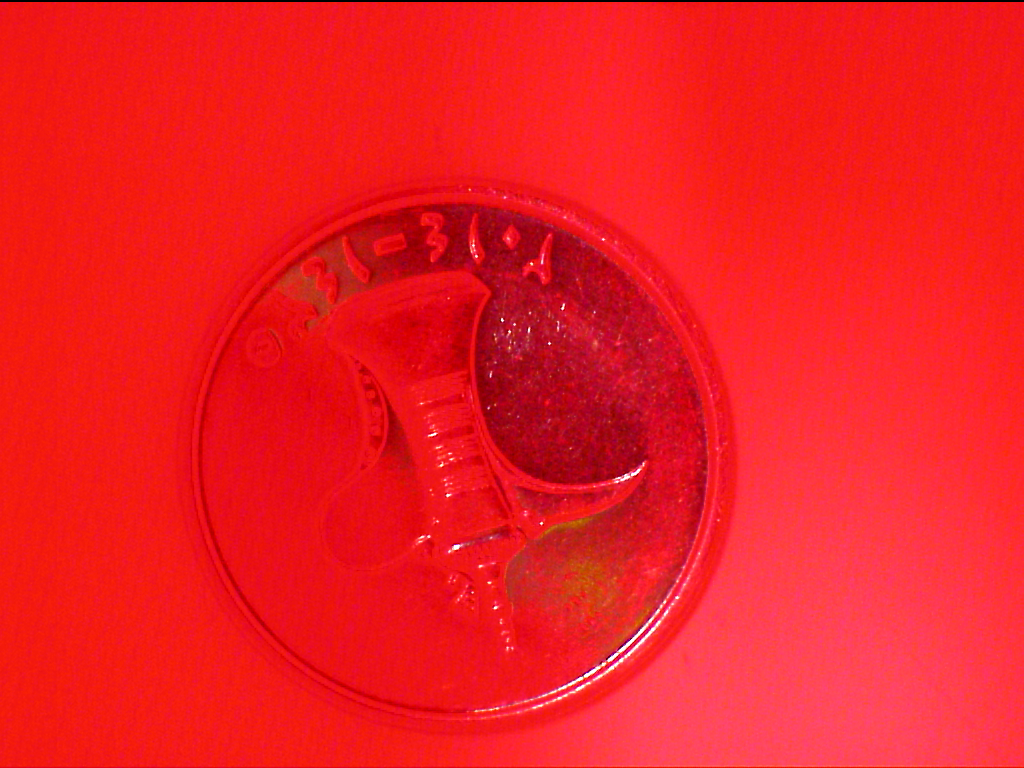
\includegraphics[width=\linewidth]{Posten_3_2_Reflektion_dom_rot}
        \caption{Mit einfallendem Streulicht}
        \label{fig:dom1}
    \end{subfigure}
    \begin{subfigure}[t]{.45\linewidth}
        
\includegraphics[width=\linewidth]{Posten_3_2_c_Reflektion_dom_rot}
        \caption{Abgedeckter Dom (kein einfallendes Streulicht, ausschliesslich Rot)}
        \label{fig:dom2}
    \end{subfigure}
\end{figure}




\clearpage
\section{Rauschen}
\subsection{Testbild ohne Belichtung}
Zunächst wurden zwei Bilder einer Identitätskarte mit maximalem Gain und ohne Beleuchtung aufgenommen. Diese sind in den Grafiken \ref{fig::imLight_1} und \ref{fig::imLight_2} ersichtlich.

\begin{figure}[ht]
	\begin{minipage}{0.45\textwidth}
		\centering
		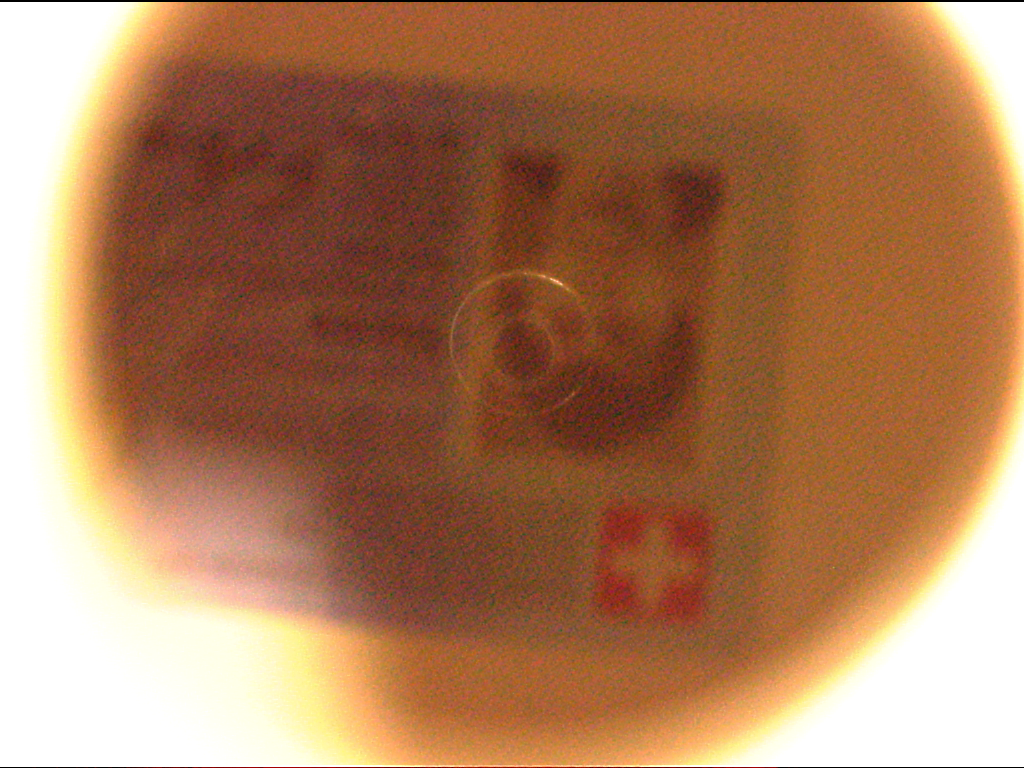
\includegraphics[width=0.8\textwidth]{Posten_4_ID_01.png}
		\caption{Erste Aufnahme der Identitätskarte}
		\label{fig::imLight_1}
	\end{minipage}
	\begin{minipage}{0.45\textwidth}
		\centering
		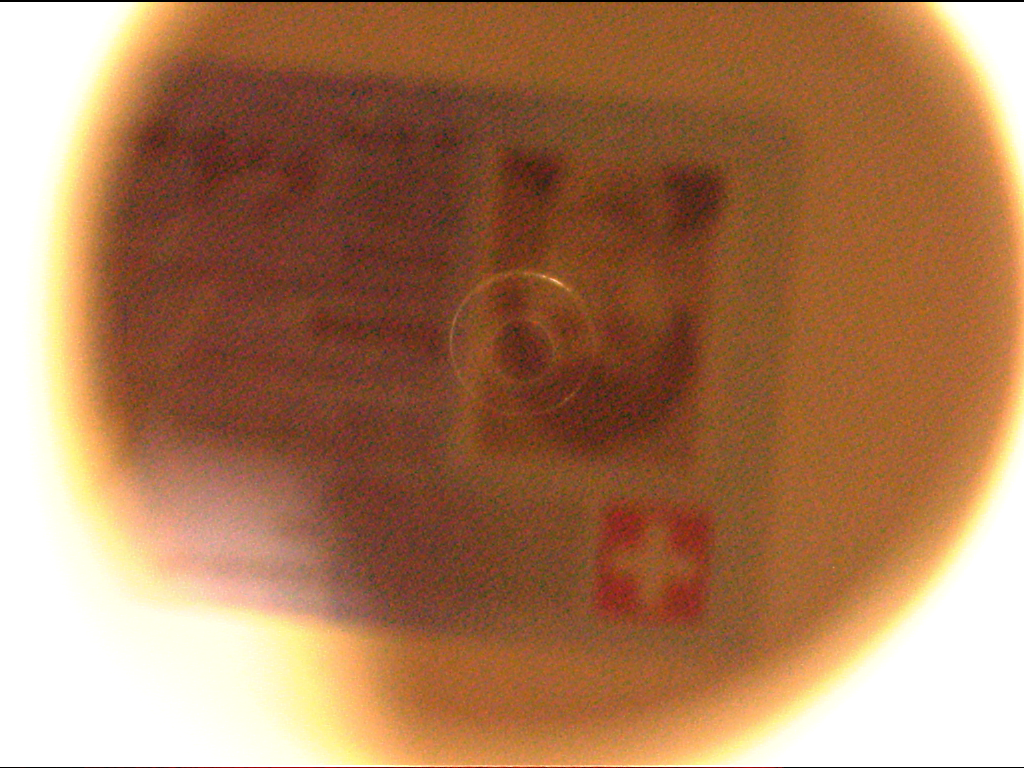
\includegraphics[width=0.8\textwidth]{Posten_4_ID_02.png}
		\caption{Zweite Aufnahme der Identitätskarte}
		\label{fig::imLight_2}
	\end{minipage}
\end{figure}

Es werden nun die beiden Bilder subtrahiert, was das Rauschen ergibt (Grafik \ref{fig::imDiff_1}). Um das Rauschen besser zu sehen wurde dieses um einen Faktor 10 verstärkt (Grafik \ref{fig::imDiff_10}).

\begin{figure}[ht]
	\begin{minipage}{0.45\textwidth}
		\centering
		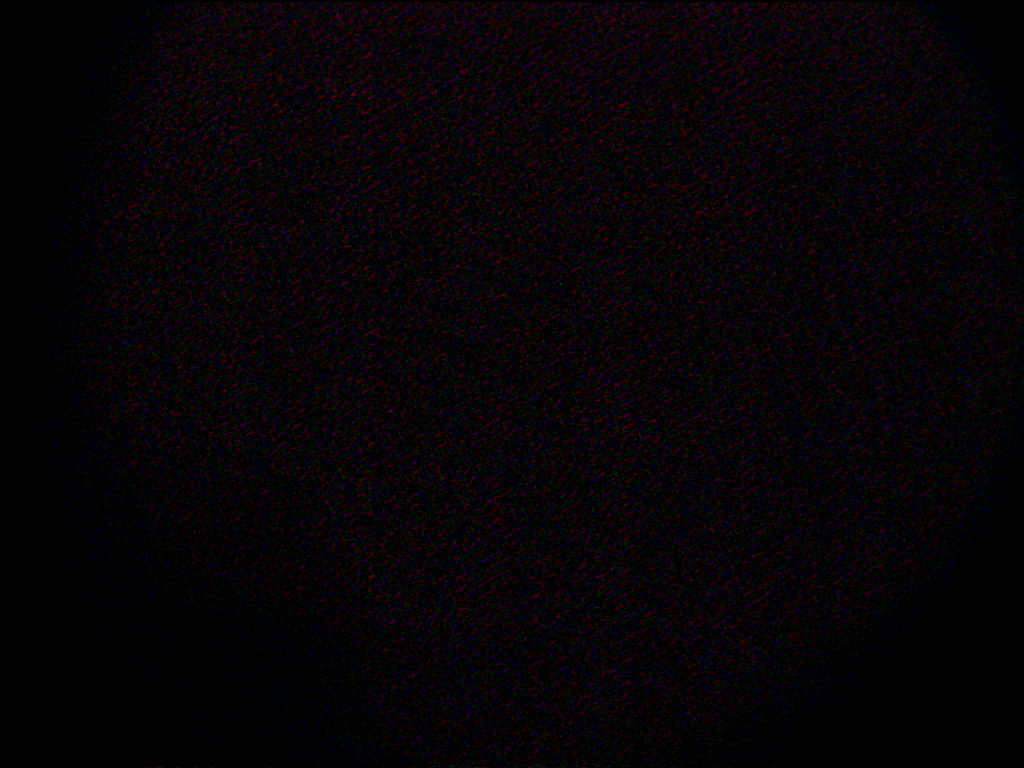
\includegraphics[width=0.8\textwidth]{imDiff_1.png}
		\caption{Unverstärktes Rauschen}
		\label{fig::imDiff_1}
	\end{minipage}
	\begin{minipage}{0.45\textwidth}
		\centering
		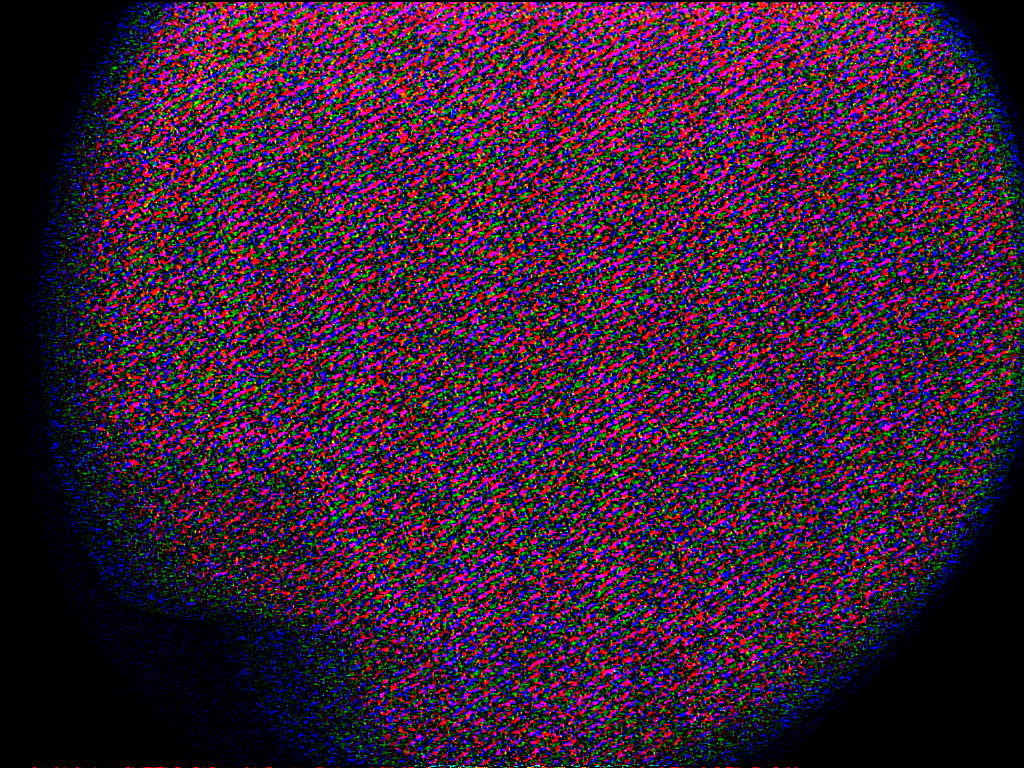
\includegraphics[width=0.8\textwidth]{imDiff_10.png}
		\caption{Verstärktes Rauschen}
		\label{fig::imDiff_10}
	\end{minipage}
\end{figure}

In der Linken Abbildung ist das unverstärkte Rauschen zu sehen, jedoch nur bei genauer Beobachtung. Deshalb wurde dies in der Rechten Abbildung verstärkt, wodurch dies wesentlich besser zu sehen ist. Dadurch ist zu sehen, dass das Rauschen im hellen Bereich des Bildes nicht vorhanden ist. Dies kommt daher, dass die Sensoren der Kamera in diesem Bereich voll ausgesteuert sind was zu einer Differenz von Null zwischen den Bildern führt.
\newpage
\subsection{Schwarzes Testbild}
Weiter wurde eine Aufnahme bei maximalem Gain und minimalen Lichteinfall gemacht, diese Aufnahme ist in Bild \ref{fig::imDead} dargestellt.

\begin{figure}[ht]
	\centering
	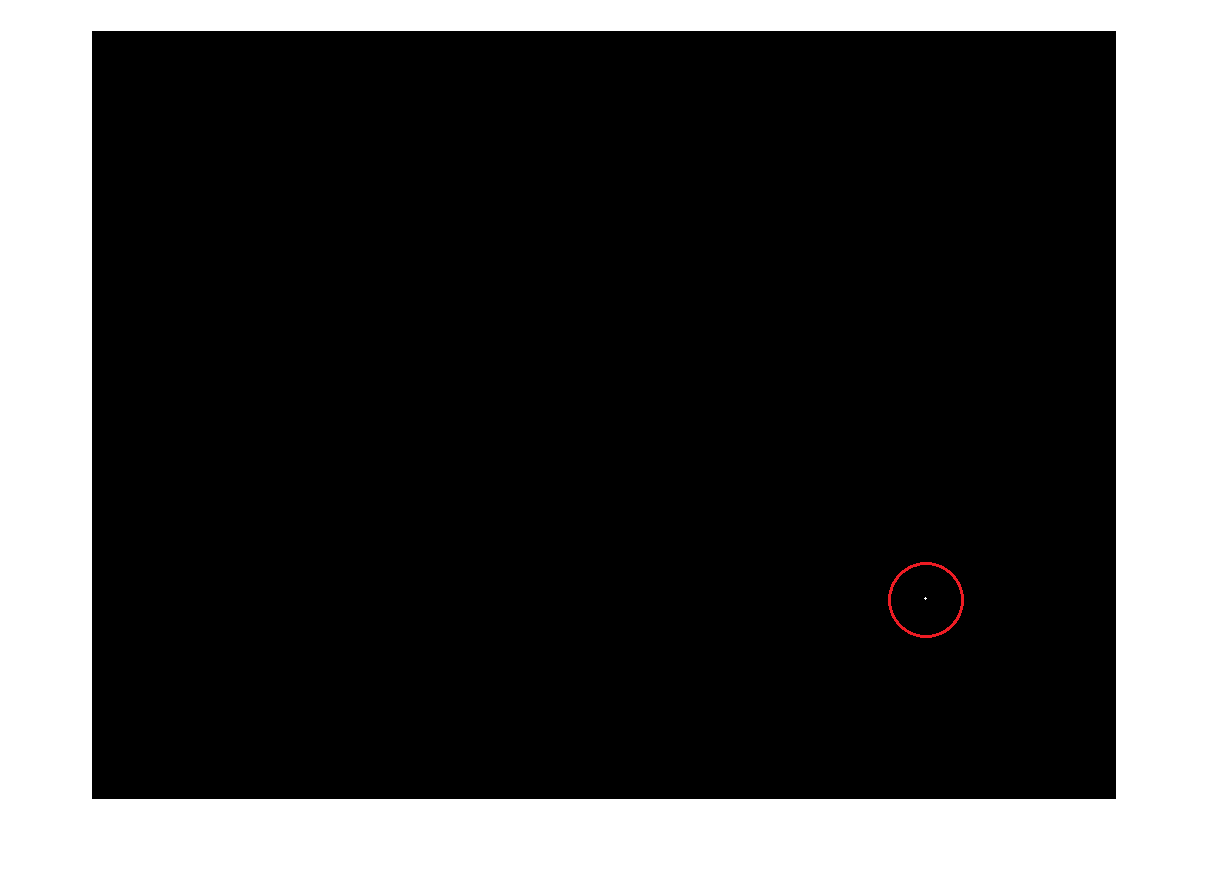
\includegraphics[width=0.8\textwidth]{imDead.png}
	\caption{Aufnahme bei minimalem Lichteinfall}
	\label{fig::imDead}
\end{figure}

In diesem Bild ist in der unteren rechten Ecke (rot markiert) der Pixelfehler der Kamera zu sehen.
\newpage
\subsection{Weisses Testbild}
Als letztes wurde noch eine Aufnahme bei beleuchtetem Dom gemacht (Grafik \ref{fig::imWhite}):

\begin{figure}[!ht]
	\centering
	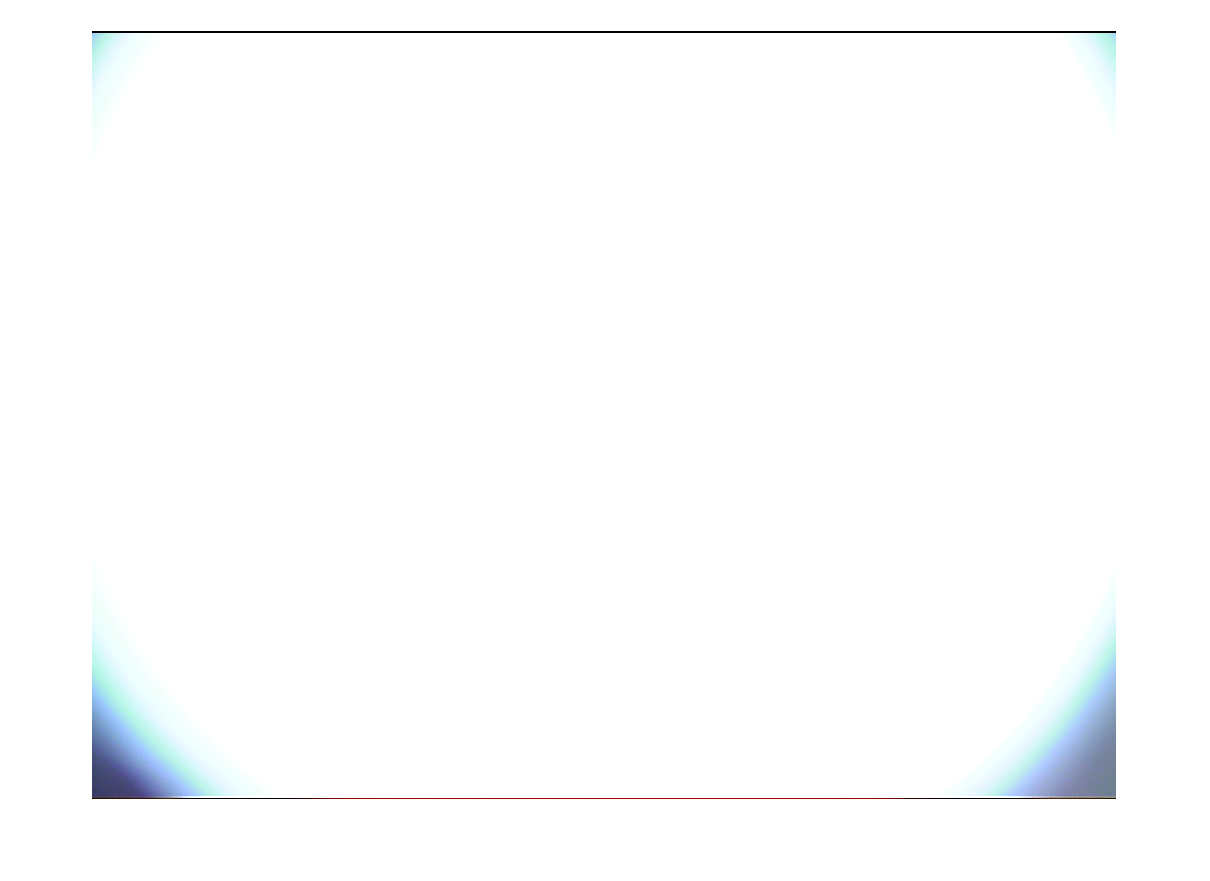
\includegraphics[width=0.8\textwidth]{imWhite.png}
	\caption{Aufnahme bei beleuchtetem Dom}
	\label{fig::imWhite}
\end{figure}

In dieser Aufnahme sollte nun die Vignettierung erkenntlich sein. Die Vignettierung ist in der Grafik jedoch nicht klar ersichtlich, weshalb darauf geschlossen werden kann, dass diese intern entfernt worden ist oder nicht ausgeprägt ist.






\clearpage
\section{Bildqualität}
\subsection{Theoretische Grundlagen}
\begin{figure}[h!]
  \centering
  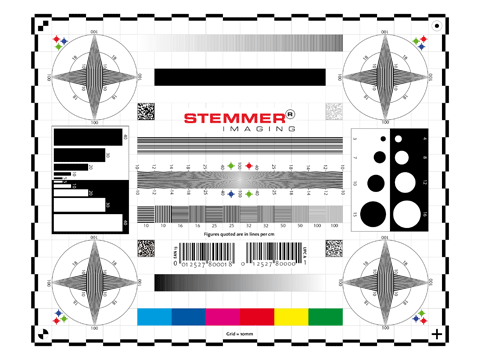
\includegraphics[width=.8\textwidth]{Posten_5_Stemmer}
  \caption{STEMMER IMAGING Test Chart for Machine Vision \cite{ref:stemmer}}
  \label{fig:p5stemmer}
\end{figure}

Die in Abbildung \ref{fig:p5stemmer} dargestellte Testchart bietet verschiedene Merkmale zur Erfassung
der Performance eines optischen Systems.
Die Chart ist mit einem $10\;\text{mm}\; \mathrm{x}\; 10\;\text{mm}$ Gitter versehen, dieses sowie die Balken links und die Kreise rechts sind zur Kalibrierung vorgesehen.

Im unteren Bereich der Chart ist ein Balken mit einem Graustufenverlauf (engl. grayscale bar).
Dieser kann verwendet werden um die Bit-Tiefe der Kamera zu bestimmen und zum Abgleich des Dynamikumfangs.

Die Barcodes (1D und 2D) sind bei diesem Versuch uninteressant.

Wichtiger sind die Quadrate mit den Strichmustern, welche mit der Anzahl Linien beschriftet sind.
Mit diesen können die Auflösung der Linse und des Bildsensors bestimmt werden.
Zum gleichen Zweck wurden die gleich darüber liegenden, zusammenlaufenden Linien angebracht.
Zusammen mit den Kompassrosen ähnlichen Segmenten in den Ecken,
kann die Performance des Linsensystems auf und abseits der optischen Achse verglichen werden.

Das Auflösungsvermögen der Optik und damit die Qualität der Linse wird durch die Modulationstransferfunktion beschrieben. Die Modulation entspricht dem Michelson Kontrast und ist folgendermassen definiert:
\begin{equation}
  M=\frac{I_{max}-I_{min}}{I_{max}+I_{min}}
\end{equation}

Die Modulationstransferfunktion ist definiert als die Abbildung von M durch das Objektiv:
\begin{equation}
  MTF=\frac{M_{Bild}}{M_{Objekt}}
\end{equation}

\newpage
\subsection{Versuchsaufbau}
Benötigtes Material:
\begin{itemize}
\item Kamera Sony DFW-X710
\item Objektiv 12.5mm
\item Testchart Stemmer-Imaging
\item Kamera Samsung Galaxy S6
\end{itemize}



\subsection{Ergebnisse}
\subsubsection{Kamera Sony DFW-X710}
\begin{figure}[h!]
  \centering
  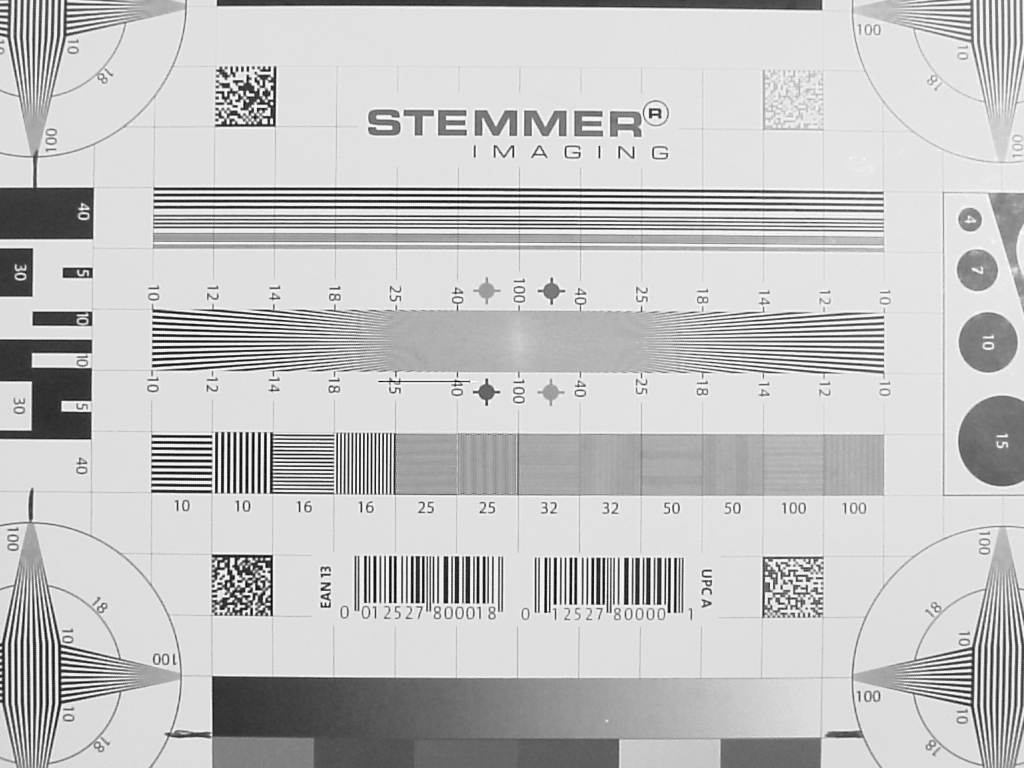
\includegraphics[width=.6\textwidth]{Posten_5_Not_so_rainbow_dildos_0}
  \caption{Graustufenbild mit Sony DFW-X710}
  \label{fig:p5g}
\end{figure}

\begin{table}[h!]
  \centering
  \begin{tabular}{l | l | l }
    Linien/10mm & Horizontal MTF &  Vertikal MTF \\\hline
    10 & 0.937 & 0.976 \\
    16 & 0.851 & 0.867 \\
    25 & 0.282 & 0.518\\
    32 & 0.169 & 0.216 \\
    50 & 0.298 & 0.200 \\
    100 & 0.271 & 0.278 \\
  \end{tabular}
\end{table}

Bei der Tabelle ist zu beachten, dass bei mehr als $\approx$25 Linien das Nyquist-Theorem verletzt wird. Die Linse ist ab diesem Punkt nicht mehr die dominierende Fehlerquelle.

\begin{figure}[H]
  \centering
  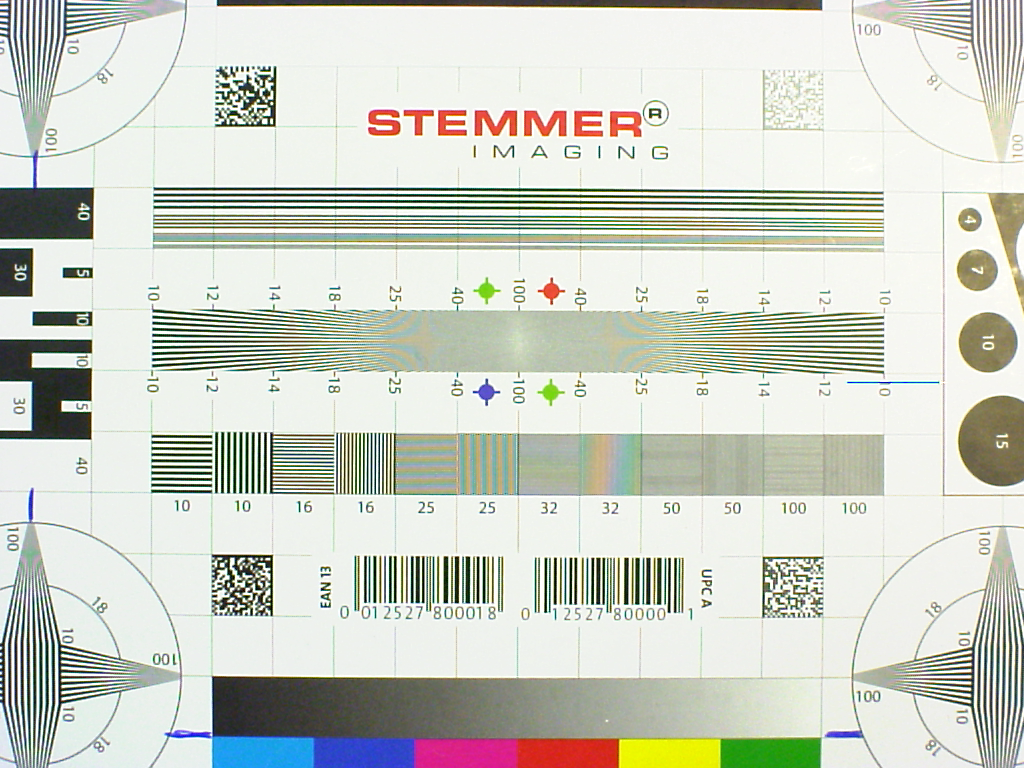
\includegraphics[width=.6\textwidth]{Posten_5_Rainbow_dildos_1}
  \caption{Farbaufname mit Sony DFW-X710}
  \label{fig:p5c}
\end{figure}

Wie in Abbildung \ref{fig:p5c} ersichtlich, sind die durch chromatische Abberation verursachten Fehler bei den Gittern mit 25 und 32 Linien durch die regebogenartige Färbung erkennbar.

\subsubsection{Kamera Samsung Galaxy S6}
\begin{figure}[h!]
  \centering
  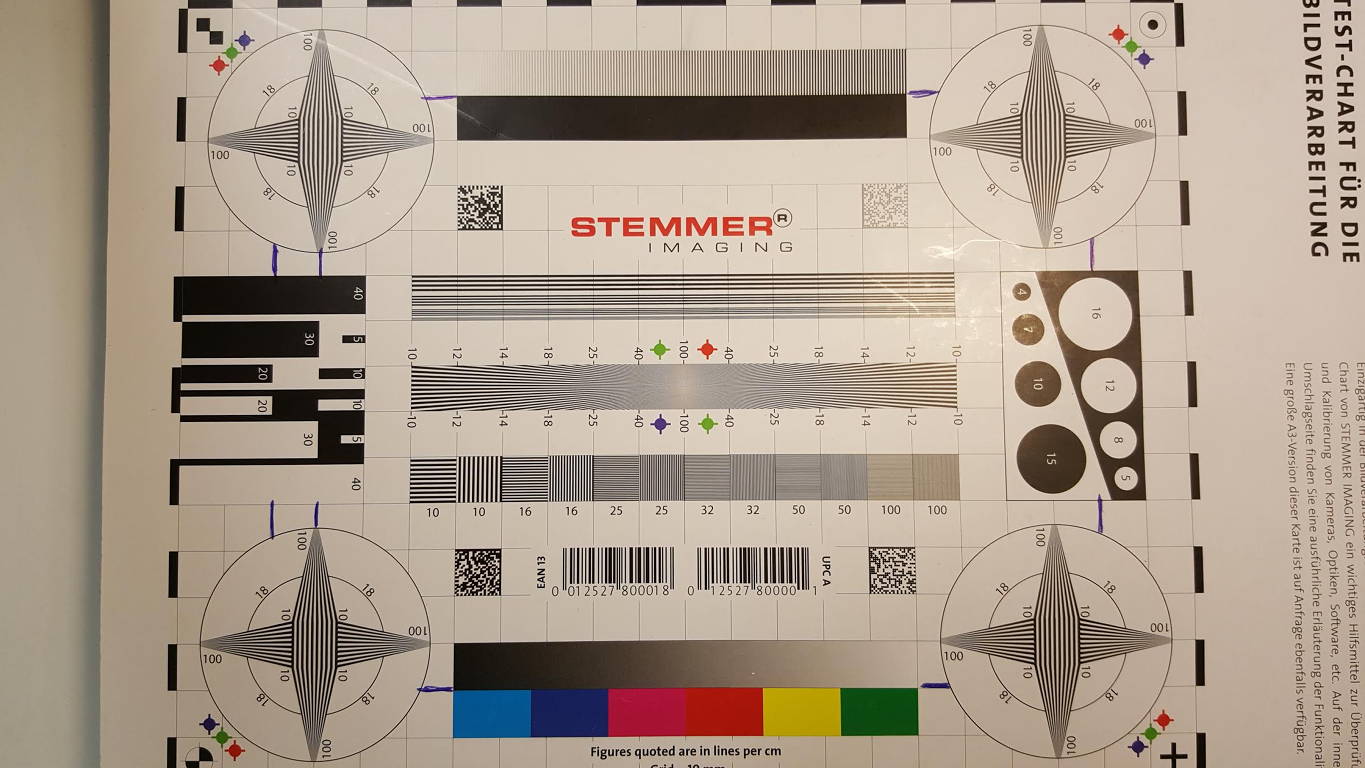
\includegraphics[width=.6\textwidth]{Posten_5_Rainbow_dildos_S6}
  \caption{Farbaufnahme mit Samsung Galaxy S6}
  \label{fig:p5s}
\end{figure}

\begin{table}[h!]
  \centering
  \begin{tabular}{l | l | l }
    Linien/10mm & Horizontal MTF &  Vertikal MTF \\\hline
    10 & 1 &  1\\
    16 & 1 & 0.992\\
    25 & 0.612 & 0.742 \\
    32 & 0.275 & 0.447 \\
    50 & 0.254 & 0.267 \\
    100 & 0.243 & 0.361 \\
  \end{tabular}
\end{table}

\newpage
\subsection{Erkenntnisse}
Wird die chromatische Abberation betrachtet, scheint die Handy Kamera deutlich besser zu sein.
Dies ist wenig erstaunlich, denn das Linsensystem beim Handy ist wesentlich kleiner, die Zahl der Fehlerquellen dementsprechend klein. Nachteile der Handy Kamera sind aber in anderen Bereichen (Zoom/Schärfentiefe) zu finden.

Zu berücksichtigen ist, dass die Aufnahm mit dem Handy nur bedingt für die Analyse der Bildqualität geeignet ist.
Die Kamera kann nur Bilder im JPEG-Format speichern, dieses reduziert die Bildgrösse
durch verlustbehaftete Komprimierung. Die Ursache eines Abbildungsfehlers kann sowohl im Optischensystem, wie auch in der digitalen Verarbeitung zu finden sein.

\begin{figure}[h!]
  \centering
  \begin{subfigure}[t]{0.49\textwidth}
    \centering
    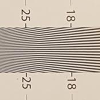
\includegraphics[width=.8\textwidth]{Posten_5_Rainbow_dildos_XXL_S6}
    \caption{JPEG komprimierte Aufnahme (Galaxy S6)}
  \end{subfigure}
  %
  \begin{subfigure}[t]{0.49\textwidth}
    \centering
    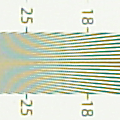
\includegraphics[width=.8\textwidth]{Posten_5_Rainbow_dildos_XXL}
    \caption{Verlustlose Aufnahme (Sony DFW-X710)}
  \end{subfigure}
  %
  \caption{Vergleich verlustbehaftete und verlustlose Kompression}
  \label{fig:p5sc}
\end{figure}

In Abbildung \ref{fig:p5sc} sind die für JPEG typischen Bildstörung besonders gut bei den Zahlen ersichtlich.

Des weiteren scheinen die Linien kurz vor der 25-er Marke die Richtung zu ändern,
ein Effekt welcher für Abtastfehler typisch ist. Der selbe Effekt tritt bei der Sony Kamera nur wenig später auf. Dies ist durch die begrenzte Auflösung erklärbar.



\clearpage
\section{Makro}
\subsection{Testbild ohne Makroring}
Für diesen Versuch sollen zwei Fotos von einer FH-Karte gemacht werden, zunächst ohne Makroring danach eine Aufnahme mit grossem Makroring, beide Aufnahmen mit einer Brennweite von 108mm.

Leider hat sich herausgestellt das die Aufnahme ohne Makroring nicht richtig abgespeichert wurde, weshalb nur die kürzeste fokussierbare Distanz von Linse zu Objekt vorhanden ist, welche 11.5cm beträgt.

\subsection{Testbild mit Makroring}
Nach dem einsetzen des Makroringes konnte dieselbe Messung nochmal gemacht werden, diesmal beträgt die gemessene Distanz von Linse zu Karte 2cm (siehe Grafik \ref{fig::imMakroring})

\begin{figure}[ht]
	\centering
	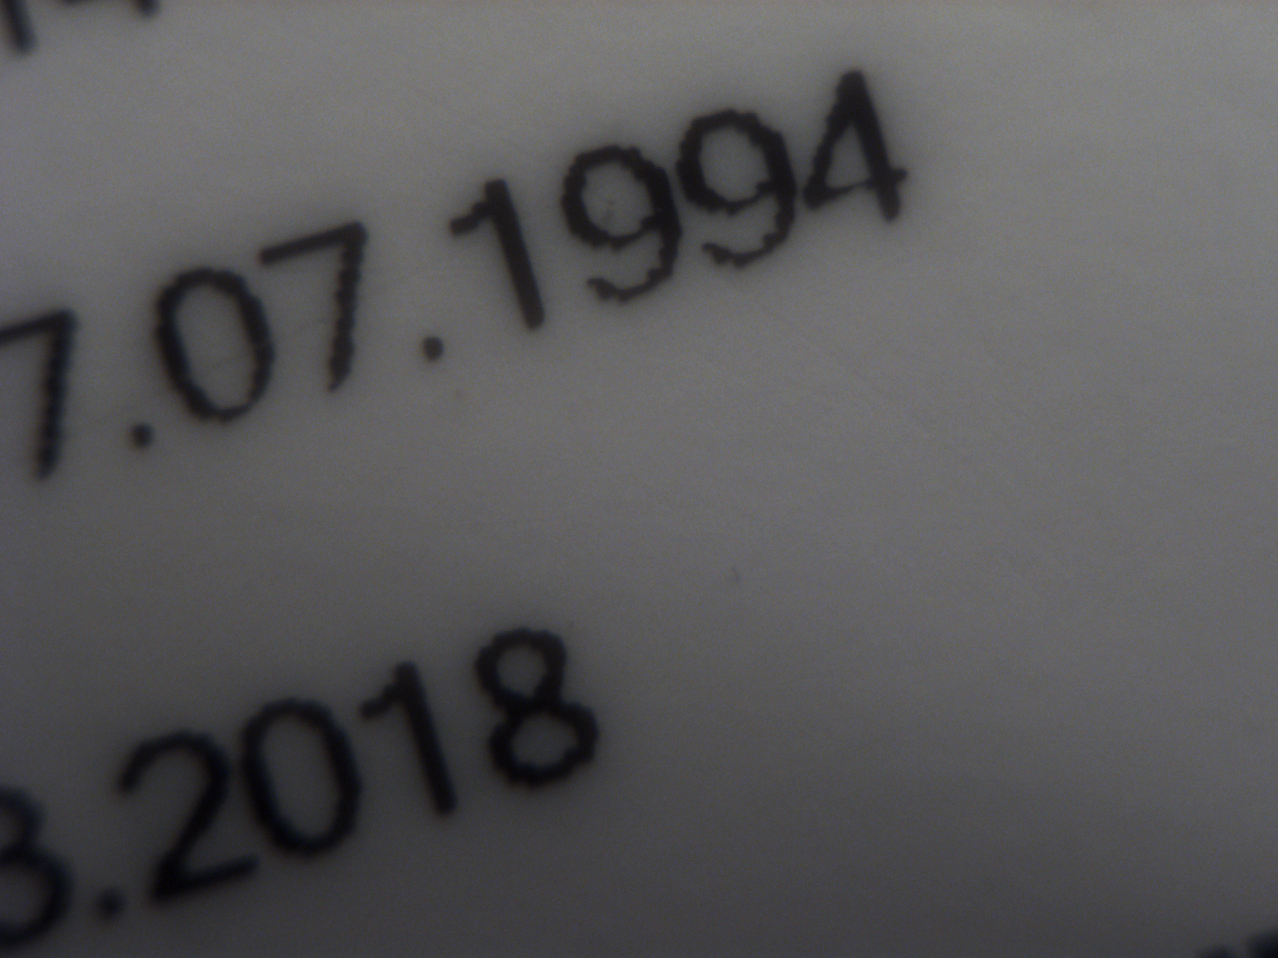
\includegraphics[width=0.8\textwidth]{imMakroring.png}
	\caption{Aufnahme mit eingesetztem Makroring}
	\label{fig::imMakroring}
\end{figure}

\subsection{Fokussieren im Unendlichen}
Als letztes wurde noch untersucht in welchem Bereich das Objekt mit Makroring fokussiert werden kann. Theoretisch sollten zwei Bereiche vorhanden sein in welchem die FH-Karte scharf zu sehen ist, es wurde aber nur der Bereich um 2cm gefunden. Es wurde die Schlussfolgerung gezogen, dass mit dem Makroring Objekte auf kürzere Distanzen scharfgestellt werden können, jedoch die maximale Distanz bei welcher ein Objekt gut zu sehen ist verringert wird

% **************************************************************************** %
% Quellenverzeichnis
% **************************************************************************** %
\clearpage
\phantomsection
\bibliographystyle{IEEEtran}
\addcontentsline{toc}{section}{\bibname}
\bibliography{bibliography}
% % **************************************************************************** %
\end{document}

